
\chapter{Arhitektura i dizajn sustava}
		 Arhitektura se može podijeliti na tri dijela:
	\begin{itemize}
		\item 	\textit{Frontend}
		\item 	\textit{Backend}
		\item 	\textit{Baza podataka}		
	\end{itemize}
		
		\underline{Frontend} predstavlja korisničko sučelje Android aplikacije i njegove funkcionalnosti. Korisničko sučelje prikazuje rezultate korisnikovih zahtjeva te olakšava njihovo slanje. Korisnik putem korisničkog sučelja šalje zahtjeve Backend-u. Korisnik može biti zaposlenik, revizor, računovođa ili direktor. Na temelju svoje uloge korisnici imaju različite ovlasti i samim time mogu slati različite zahtjeve.
		HTTP zahtjevi se šalju na Amazon AWS API Gateway koji je zadužen za obradu zahtjeva. API Gateway zatim prosljeđuje zahtjev backend-u.\\
		
		\underline{Backend} predstavlja dio programa koji se izvodi na web poslužitelju i omogućava izvršavanje zahtjeva koje korisnik šalje. Komunikacija Frontend-a i Backend-a odvija se HTTP protokolom. Nakon što Backend primi zahtjev koji je korisnik uputio, on iz njega izlučuje podatke potrebne za izvršavanje zahtjeva. Ti podaci nalaze se u body-ju HTTP zahtjeva. Backend je ostvaren korištenjem Amazon AWS Lambde. Za svaku vrstu zahtjeva stvorena je zasebna Lambda. Svaka Lambda sadrži funkciju koja kao argument prima body HTTP zahtjeva u obliku rječnika u kojem su ključevi nazivi parametara koji se se šalju zahtjevom. Zatim se izvrši kod funkcije i njena povratna vrijednost se ponovo šalje korisniku na frontend-u preko API Gateway-a. Funkcije u Lambdi koriste Psycopg2 adapter za slanje zahtjeva na bazu podataka. \\
		
		U \underline{bazi podataka} nalaze se podaci o korisnicima i dokumenti koje su skenirali. Baza je napravljena koristeci Amazon AWS RDS.\\\\\\
		
		Za izradu Frontend-a naše android aplikacije izabrali smo programski jezik Java, a za Backend smo koristili Python. Za razvoj Frontend-a koristili smo Android Studio, a za razvoj Backend-a Visual Studio Code razvojno okruženje.\\
	
		Raspodjela arhitekture na Frontend, Backend i bazu podataka omogućila je lakše ispitivanje pojedinih dijelova sustava kao i jednostavnije i nezavisnije razvijanje.
		
		
		\begin{figure}
			\centering
			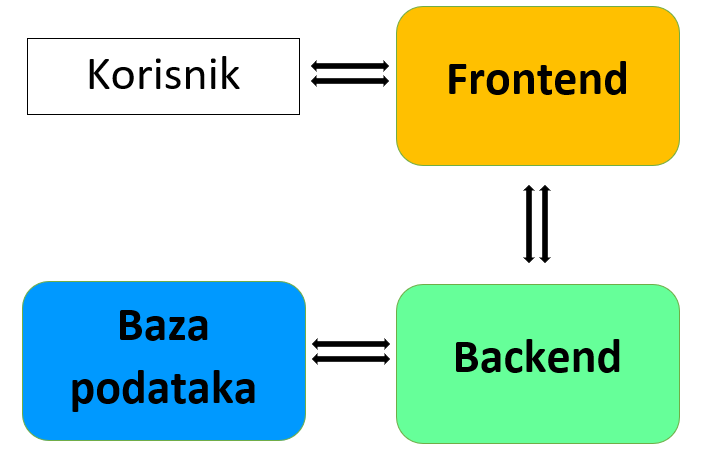
\includegraphics[scale=0.75]{./slike/Prikaz arhitekture.png}
			\caption{Arhitektura sustava}
			\label{fig:ARH}
		\end{figure}
		

		


		\section{Baza podataka}
			
			
			
		Koristili smo relacijsku bazu podataka koju smo napravili u postgreSQL-u.\\
		Trenutna početna verzija baze sadrži relaciju users.
		
			\subsection{Opis tablica}
			

			
				
				
				\begin{longtblr}[
					label=none,
					entry=none
					]{
						width = \textwidth,
						colspec={|X[8,l]|X[8, l]|X[20, l]|}, 
						rowhead = 1,
					} %definicija širine tablice, širine stupaca, poravnanje i broja redaka naslova tablice
					\hline \multicolumn{3}{|c|}{\textbf{users}}	 \\ \hline[3pt]
					\SetCell{LightGreen}userId & SERIAL	&  	Jedinstveni identifikator korisnika  	\\ \hline
					firstName	& VARCHAR(50) & Ime korisnika   	\\ \hline 
					lastName & VARCHAR(50) & Prezime korisnika   \\ \hline 
					username & VARCHAR(50)	& Korisničko ime korisnika - jedinstveno  		\\ \hline 
					userPswd & VARCHAR(50) & Lozinka korisnika  \\ \hline
					 userRole & VARCHAR(20) & Uloga korisnika   	\\ \hline 
				\end{longtblr}
				
			U tablici users zapisani su svi korisnici aplikacije, svaki korisnik ima jedinstveno korisničko ime (username) i dodjeljuje mu se jedinstveni identifikator (userId) koji je primarni ključ tablice.
			Ostali atributi koje svaki korisnik ima su njegovo ime i prezime, lozinka u aplikaciji (za prijavu mora unijeti korisničko ime i lozinku) i uloga unutar tvrtke.
			
			
					\begin{longtblr}[
					label=none,
					entry=none
					]{
						width = \textwidth,
						colspec={|X[8,l]|X[8, l]|X[20, l]|}, 
						rowhead = 1,
					} %definicija širine tablice, širine stupaca, poravnanje i broja redaka naslova tablice
					\hline \multicolumn{3}{|c|}{\textbf{scanHistory}}	 \\ \hline[3pt]
					\SetCell{LightGreen}docId & SERIAL &  Jedinstveni identifikator dokumenta  	\\ \hline
					\SetCell{LightBlue}userId & INT & Identifikator korisnika  	\\ \hline 
					scanDate & DATE & Datum skeniranja  \\ \hline 
				\end{longtblr}
			scanHistory je tablica koja u sebi sadrži sve skenirane dokumente, bili oni ispravno ili neispravno skenirani, ispravno skenirani dokumenti će otići u documents dok će neispravni samo ostati ovdje.
			Njeni atributi su docId (jedinstveni identifikator svakog skeniranog dokumenta), userId (jedinstveni identifikator korisnika koji je skenirao dokument) i datum skeniranja
			
				\begin{longtblr}[
				label=none,
				entry=none
				]{
					width = \textwidth,
					colspec={|X[8,l]|X[8, l]|X[20, l]|}, 
					rowhead = 1,
				} %definicija širine tablice, širine stupaca, poravnanje i broja redaka naslova tablice
				\hline \multicolumn{3}{|c|}{\textbf{documents}}	 \\ \hline[3pt]
				\SetCell{LightGreen}docId & INT	&  	Jedinstveni identifikator dokumenta  	\\ \hline
				docLabel & VARCHAR(10) & Oznaka dokumenta   	\\ \hline 
				docType & VARCHAR(1) & Tip dokumenta   	\\ \hline 
				docText & TEXT & Skenirani tekst   \\ \hline 
			\end{longtblr}
		Tablica documents sadrži podatke o svim dokumentima koji su potvrđeni kao ispravno skenirani, podaci koji su zapisani u njoj su docId (jedinstveni identifikator), docLabel (oznaka dokumenta), docType (tip dokumenta) i docText (skenirani tekst u dokumentu) 
		


\begin{longtblr}[
	label=none,
	entry=none
	]{
		width = \textwidth,
		colspec={|X[8,l]|X[8, l]|X[20, l]|}, 
		rowhead = 1,
	} %definicija širine tablice, širine stupaca, poravnanje i broja redaka naslova tablice
	\hline \multicolumn{3}{|c|}{\textbf{accountantResponsibility}}	 \\ \hline[3pt]
	\SetCell{LightGreen}userId & INT & Identifikator korisnika  	\\ \hline 
	responsibility & VARCHAR(1) & Zaduženje računovođe (Računi, ponude ili interni dokumenti)  \\ \hline 
	
\end{longtblr}

accountantResponsibility je tablica koja u sebi sadrži userId nekog računovođe i njegovo zaduženje (računi, ponude ili interni dokumenti)


\begin{longtblr}[
	label=none,
	entry=none
	]{
		width = \textwidth,
		colspec={|X[8,l]|X[8, l]|X[20, l]|}, 
		rowhead = 1,
	} %definicija širine tablice, širine stupaca, poravnanje i broja redaka naslova tablice
	\hline \multicolumn{3}{|c|}{\textbf{archive}}	 \\ \hline[3pt]
	\SetCell{LightGreen}archiveId & SERIAL &  Jedinstveni identifikator arhive  	\\ \hline
	\SetCell{LightBlue}docId & INT & Jedinstveni identifikator dokumenta  \\ \hline 
	\SetCell{LightBlue}userId & INT & Identifikator korisnika \\ \hline
	archivedDate & DATE & Datum arhiviranja \\ \hline
	signed & SMALLINT & Dokument potpisan/nepotpisan \\ \hline
	
\end{longtblr}

archive je tablica u koju se spremaju svi dokumenti koje računovođe arhiviraju,
svaka arhiva ima svoj jedinstveni identifikator (archiveId).
Atributi koji se spremaju uz archiveId su docId arhiviranog dokumenta, userId računovođe koji ga je arhivirao, datum arhiviranja i signed (dokument potpisan/ne)

\begin{longtblr}[
	label=none,
	entry=none
	]{
		width = \textwidth,
		colspec={|X[8,l]|X[8, l]|X[20, l]|}, 
		rowhead = 1,
	} %definicija širine tablice, širine stupaca, poravnanje i broja redaka naslova tablice
	\hline \multicolumn{3}{|c|}{\textbf{reviserPending}}	 \\ \hline[3pt]
	\SetCell{LightGreen}docId & INT &  Jedinstveni identifikator dokumenta  	\\ \hline
	\SetCell{LightBlue}userId & INT & Identifikator korisnika  	\\ \hline 
	
\end{longtblr}

reviserPending je tablica u koju se spremaju dokumenti koji se šalju revizoru, kad će revizor potvrđivati i proslijeđivati dokumente, pregledavati će dokumente iz ove tablice.
Ima samo 2 atributa, a to su docId dokumenta kojeg je zaposlenik poslao i userId revizora kojem se šalje taj dokument. 


\begin{longtblr}[
	label=none,
	entry=none
	]{
		width = \textwidth,
		colspec={|X[8,l]|X[8, l]|X[20, l]|}, 
		rowhead = 1,
	} %definicija širine tablice, širine stupaca, poravnanje i broja redaka naslova tablice
	\hline \multicolumn{3}{|c|}{\textbf{executivePending}}	 \\ \hline[3pt]
	\SetCell{LightGreen}docId & INT &  Jedinstveni identifikator dokumenta  	\\ \hline
	\SetCell{LightBlue}userId & INT & Identifikator korisnika  	\\ \hline 
	
\end{longtblr}

executivePending je tablica u koju se spremaju dokumenti koje računovođe šalju direktoru na potpis prije arhiviranja,
isto ima samo 2 atributa, a to su docId dokumenta poslanog na potpis i userId računovođe kojem se potpisani dokument treba vratiti. 


\begin{longtblr}[
	label=none,
	entry=none
	]{
		width = \textwidth,
		colspec={|X[8,l]|X[8, l]|X[20, l]|}, 
		rowhead = 1,
	} %definicija širine tablice, širine stupaca, poravnanje i broja redaka naslova tablice
	\hline \multicolumn{3}{|c|}{\textbf{accountantPending}}	 \\ \hline[3pt]
	\SetCell{LightGreen}docId & INT &  Jedinstveni identifikator dokumenta  	\\ \hline
	\SetCell{LightBlue}userId & INT & Identifikator korisnika  	\\ \hline 
	signaturePending & SMALLINT & Status potpisa  	\\ \hline 
	
\end{longtblr}

accountantPending je tablica u koju se spremaju dokumenti koji se šalju računovođi na arhiviranje.\\
Računovođa kojem će dokument biti dostavljen je odabran s obzirom na svoju odgovornost (tablica accountantResponsibility), atributi tablice accountantPending su docId dokumenta koji je poslan računovođi, userId računovođe kojem je poslan dokument i atribut signaturePending koji govori je li potpis tražen.\\
Ako je vrijednost atributa signaturePending 0, potpis nije tražen, ako je 1, potpis je tražen, ali direktor još nije potpisao dokument, a ako je 2, onda je potpis tražen i direktor je potpisao i vratio dokument. 




			
			\subsection{Dijagram baze podataka}
			
			\eject
			\begin{figure}
				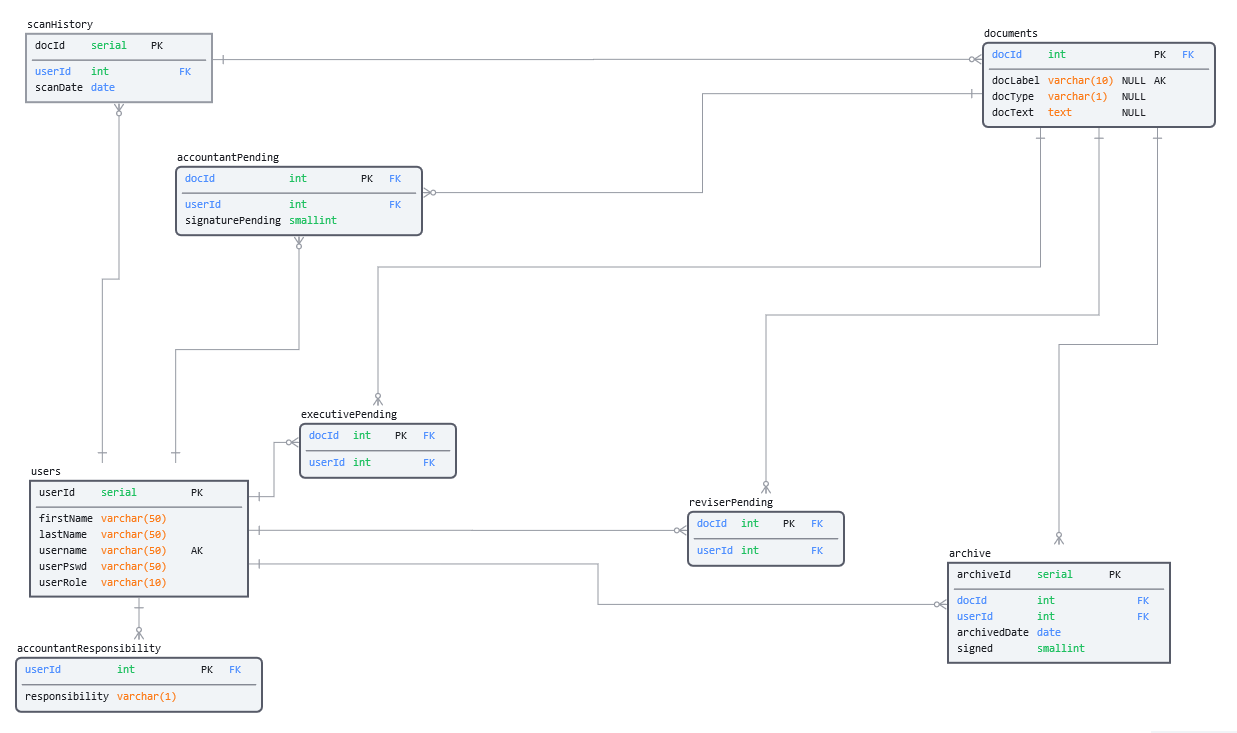
\includegraphics[width=\linewidth]{./dijagrami/ER.png}
				\caption{ER Diagram}
				\label{fig:ER}
			\end{figure}
			
			
		\section{Dijagram razreda}
			
			Na slici su prikazani razredi koji pripadaju backend dijelu MVC
			arhitekture.\\
			U izvornom kodu postoje samo razredi \textit{User} i \textit{Document}.\\ Razred \textit{User} ima atribut \textit{role} koji određuje kojim funkcijama "handlerima" instanca razreda ima pristup. Postoje tri tipa računovođa koji imaju pristup istim funkcijama. Jedina je razlika u tipu dokumenta kojega arhiviraju.\\
			Razred \textit{Document} ima atribut \textit{type} koji određuje tip dokumenta, te kojem računovođi se šalju. Svi tipovi imaju pristup jednakim funkcijama "handlerima".\\
			Različiti atributi \textit{role} i \textit{type} su u dijagramu prikazani kao razredi izvedeni iz razreda \textit{User} radi preglednosti.\\
			
			\begin{figure}
				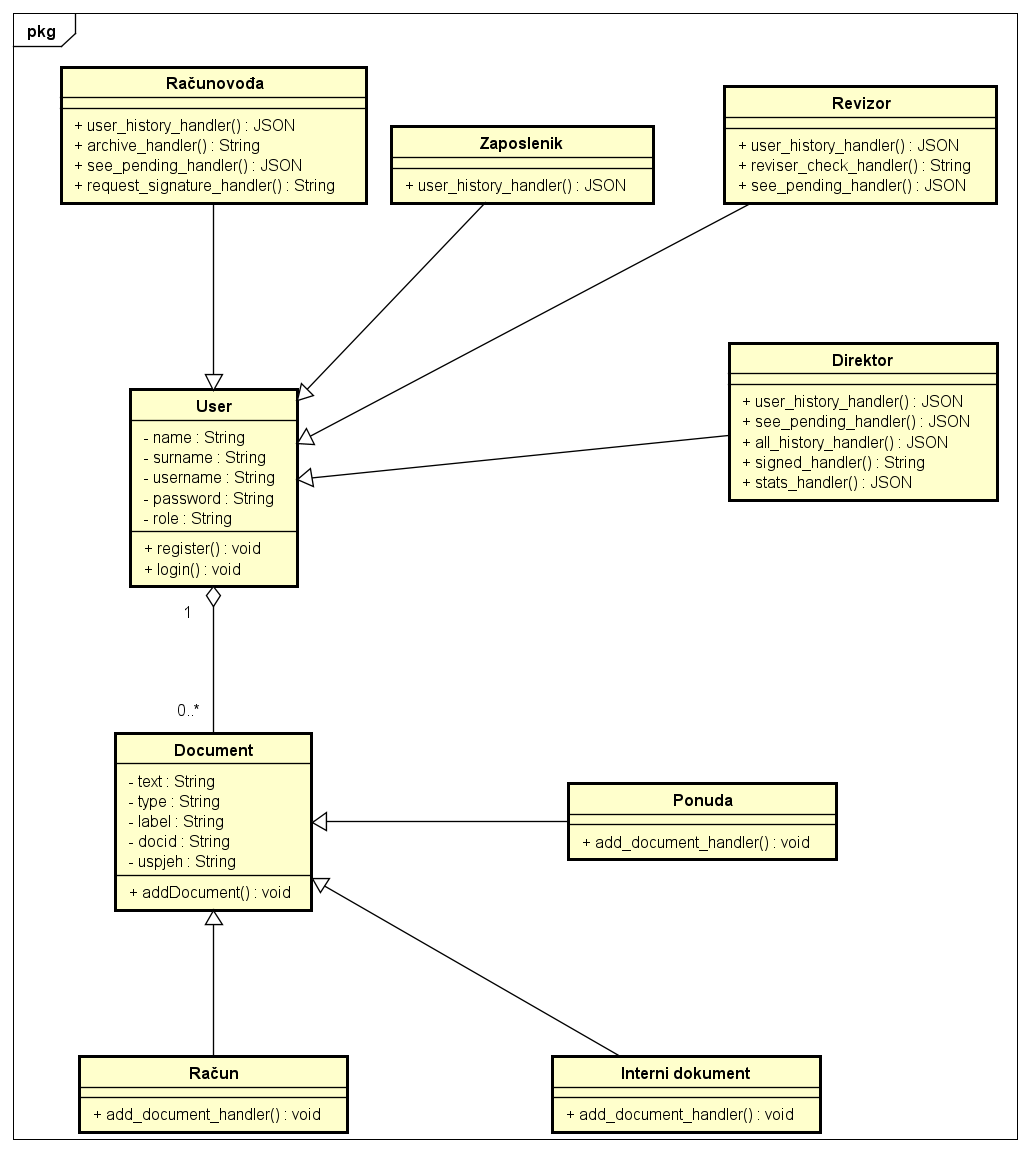
\includegraphics[width=\linewidth]{./dijagrami/dijagram_razreda.png}
				\caption{Dijagram razreda}
				\label{fig:Class}
			\end{figure}
			
			
			
			\eject
		
		\section{Dijagram stanja}
			
			
		
			
			U nastavku je dijagram stanja koji prikazuje stanja, odnosno "stranice" aplikacije. 
			Također su i naznačeni trenutci  u kojima aplikacija komunicira s back-endom. Uvedena je simplifikacija glavne aktivnosti zaposlenika, revizora, direktora i računovođe u glavnu aktivnost radi jednostavnijeg prikaza.
			
			\bigskip
			\bigskip
			\bigskip
			
			\begin{figure}[H]
				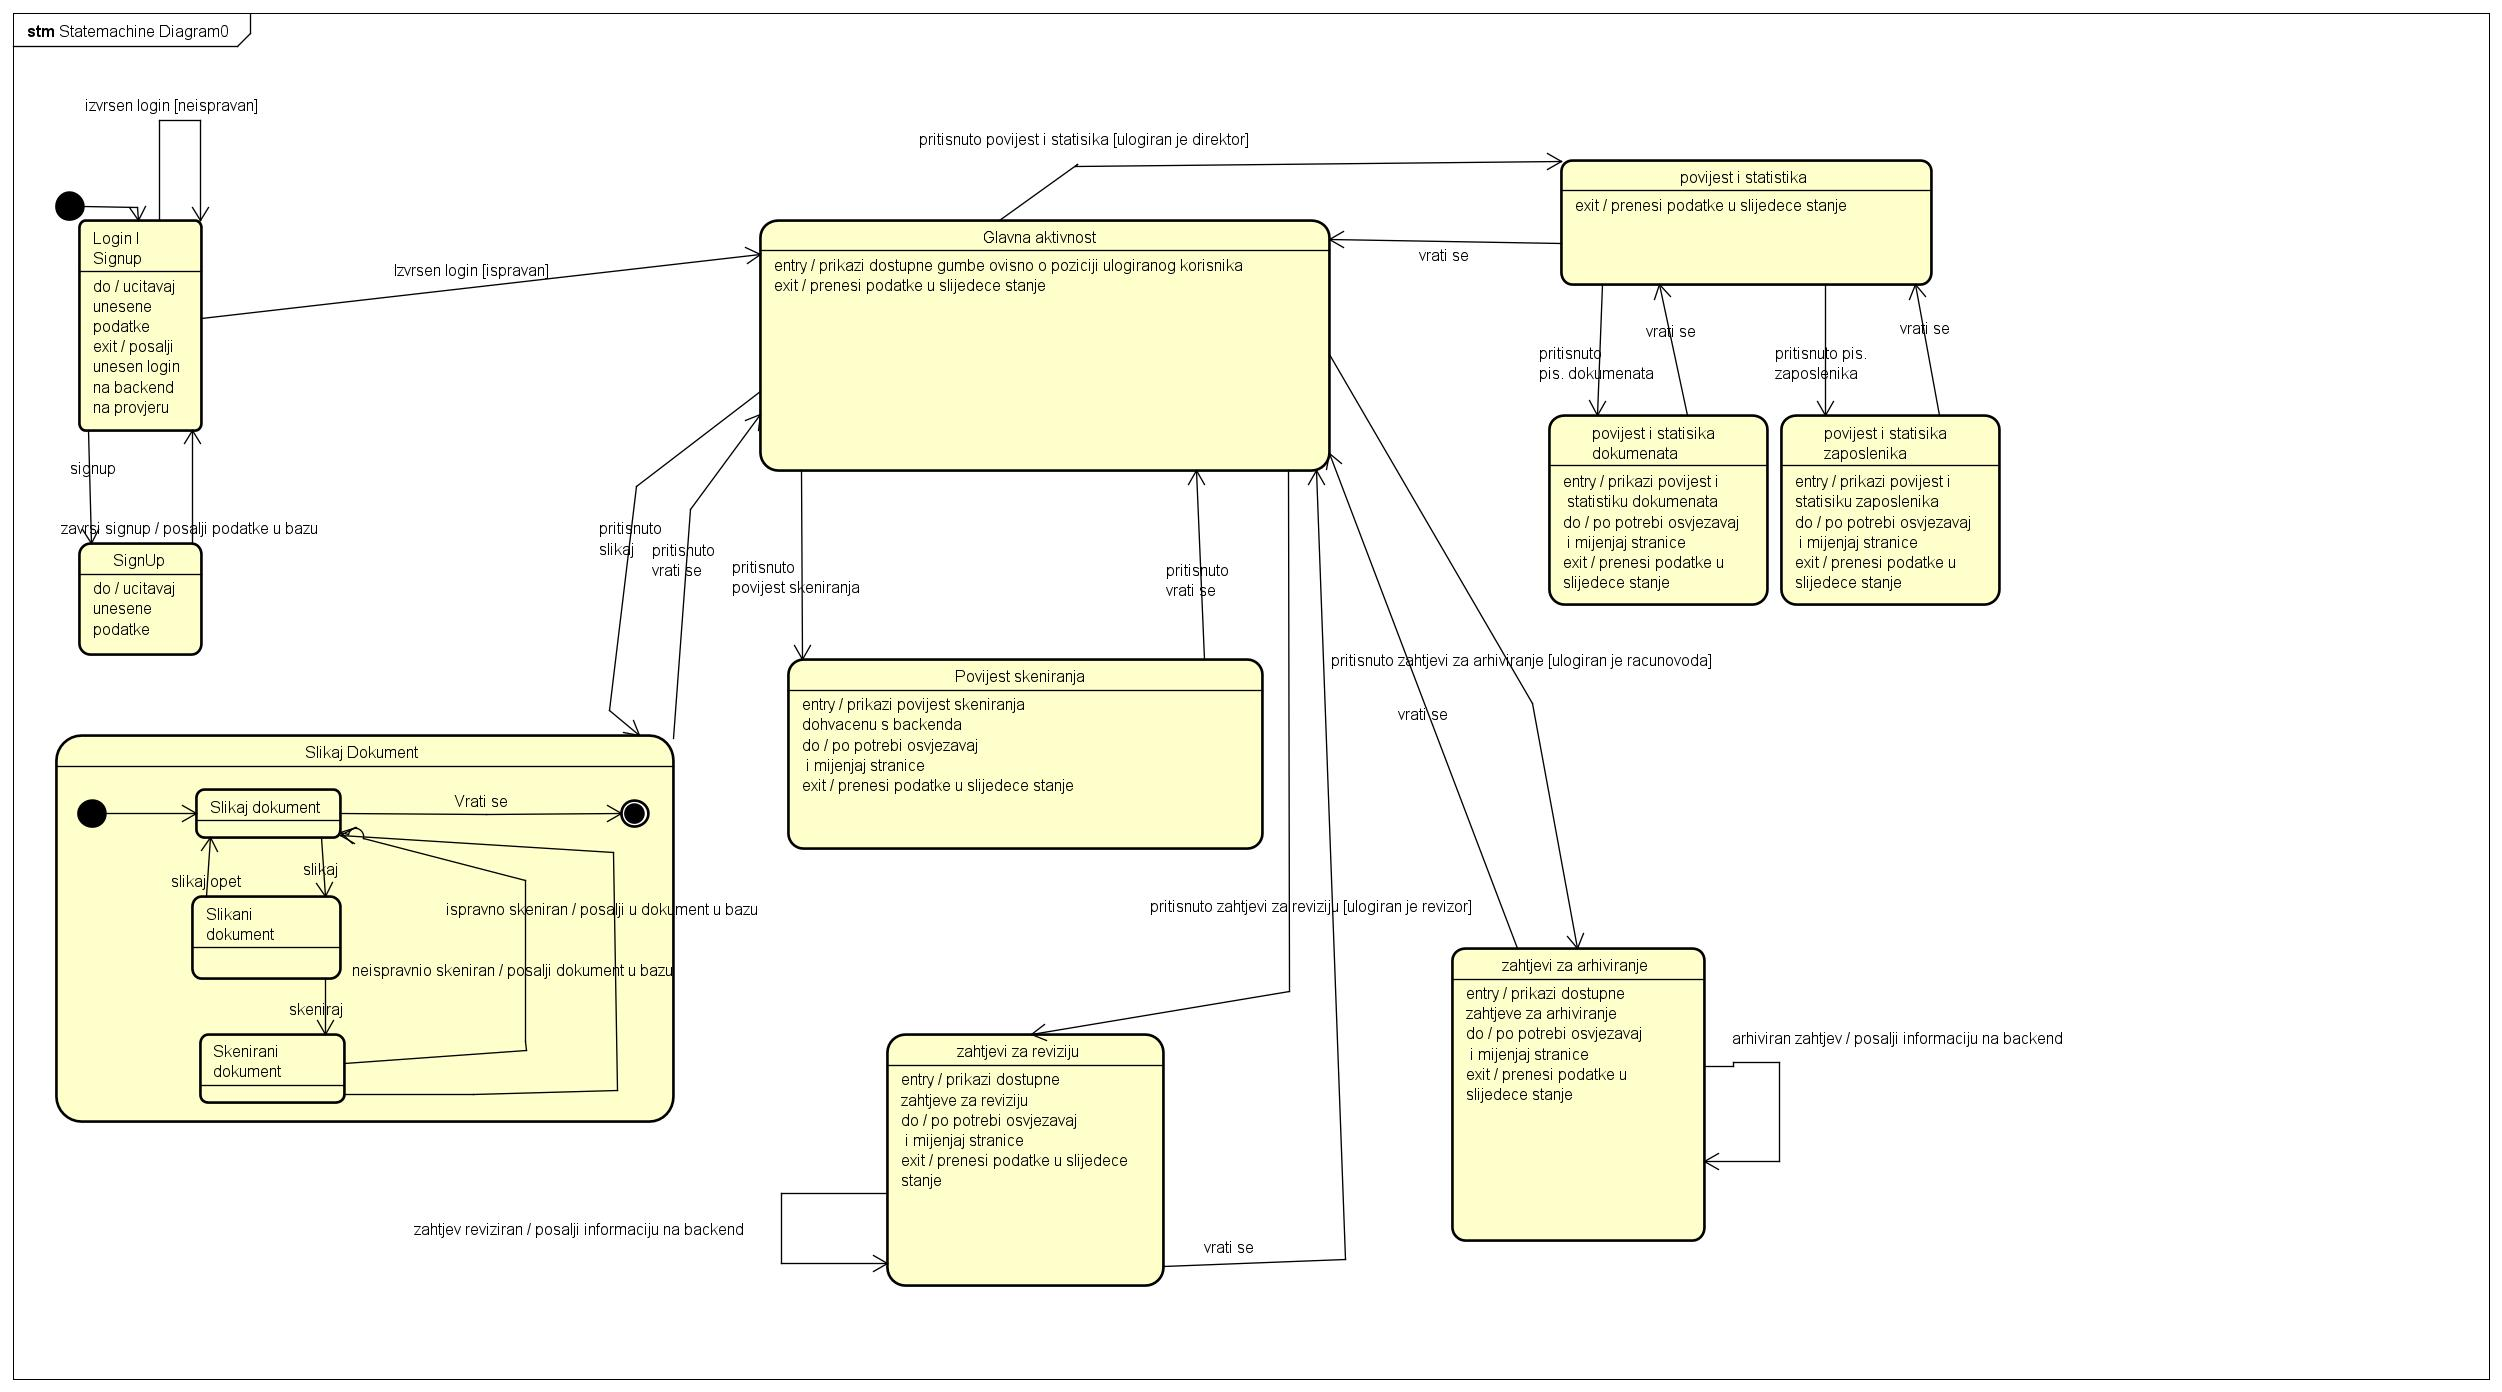
\includegraphics[width=\linewidth]{./dijagrami/Dijagram_stanja.jpg}
				\caption{Dijagram stanja}
				\label{fig:Class}
			\end{figure}
			
			\eject 
		
	\section{Dijagram aktivnosti}
	
	
	
	Dijagram aktivnosti pokazuje proces skeniranja jednog dokumenta.
		Korisnik se prvo prijavljuje u svoj korisnički račun gdje
		odabire funkciju skeniranja. Zatim korisnik slika željeni dokument i aplikacija mu prikazuje dobiveni sažetak dokumenta. 
		Korisnik završno odlučuje jeli zadovoljan sa sažetkom te se taj njegov odgovor i sažetak šalju u bazu podataka čime je završen proces skeniranja.
	
	
	\begin{figure}
		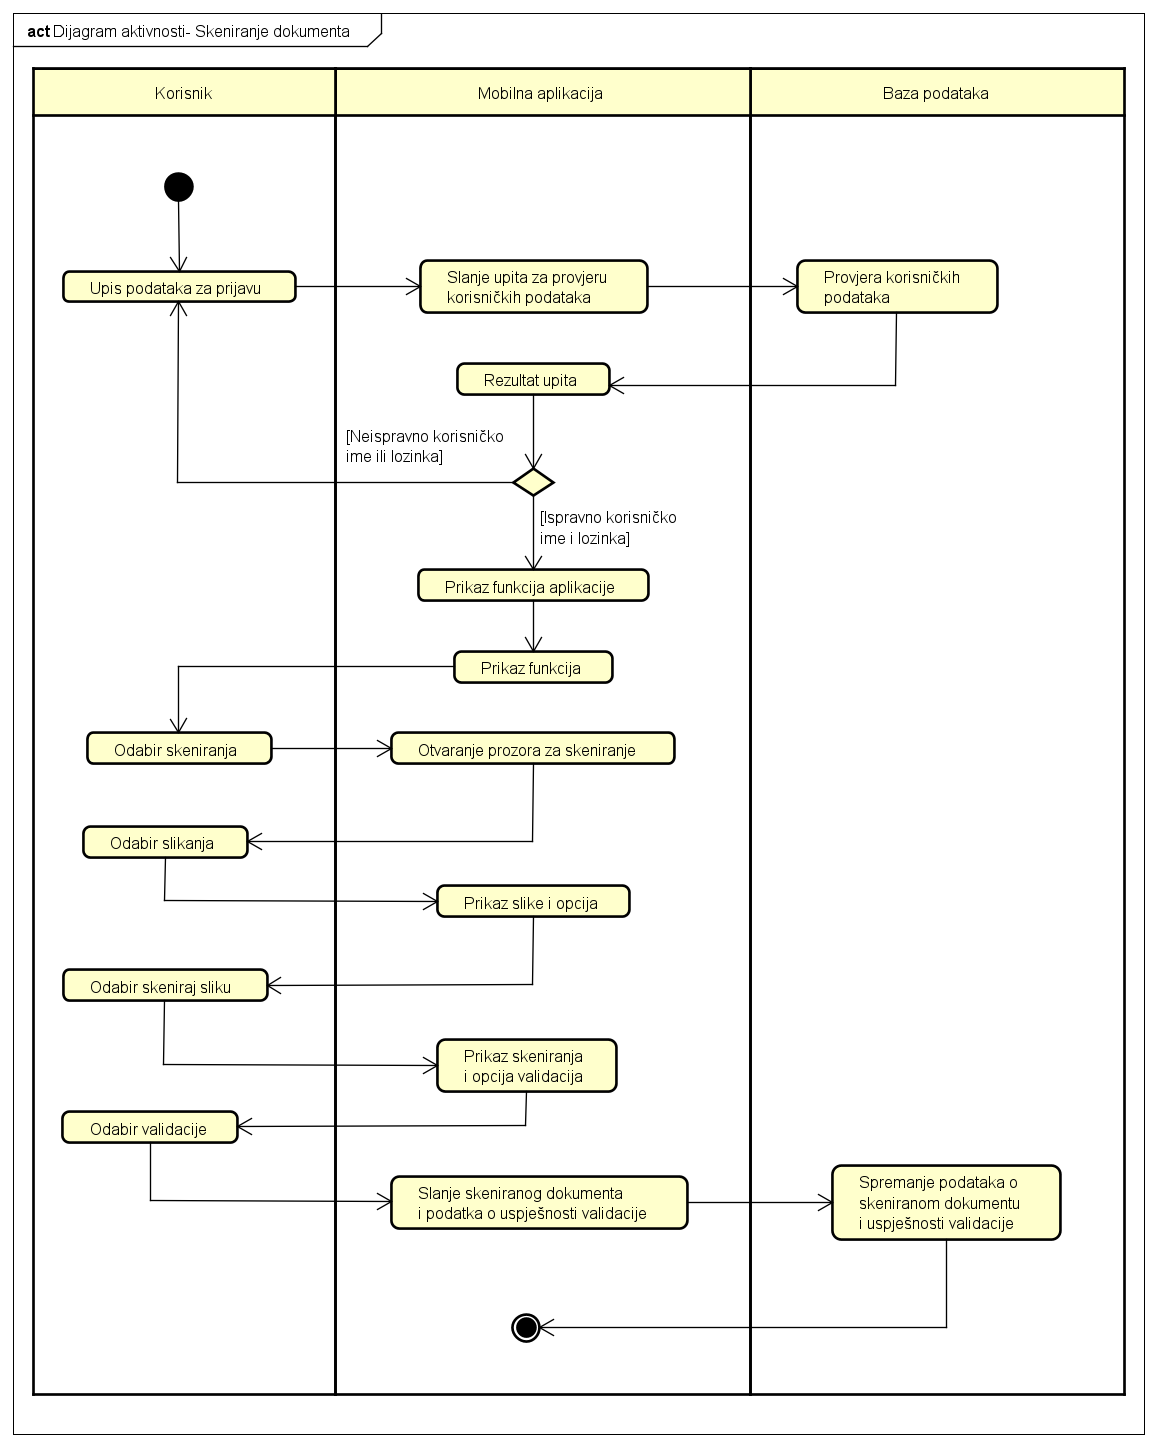
\includegraphics[width=\linewidth]{./dijagrami/dijagram_aktivnosti.png}
		\caption{Dijagram aktivnosti - Skeniranje dokumenta}
		\label{fig:Aktivnost}
	\end{figure}
	
	\eject
		\section{Dijagram komponenti}
		
			\textbf{\textit{dio 2. revizije}}\\
		
			
			 
			 Dijagram komponenti na slici 4.4 prikazuje komponente sustava te njihove međuovisnosti. Sustavu se pristupa preko komponente grafičkog sučelja koja je zadužena za prikaz sadržaja korisniku. Glavna funkcionalnost aplikacije jest mogućnost skeniranja dokumenata i njihovo spremanje u bazu podataka. Zato je grafičkom sučelju potreban API koji će mu omogućiti prepoznavanje teksta te mu je potrebno sučelje za komunikaciju s poslužiteljem, a sam nudi sučelje za slanje podataka u obliku JSON objekata. Komponenta "OCR prepoznavanje teksta" nudi sučelje za skeniranje dokumenata dok se komunikacija s poslužiteljem odvija "Dohvati JSON" i "Šalje JSON" sučelja. Komponenta "Lambda API Gateway" je zadužena za komunikaciju s bazom podataka i s grafičkim sučeljem, a za rad su joj potrebne komponente "Dokument" i "Korisnik" kako bi mogla komunicirati s bazom podataka. Baza podataka nudi sučelje preko kojeg je omogućena komunikacija s poslužiteljem.
			 
			 \begin{figure}[H]
			 	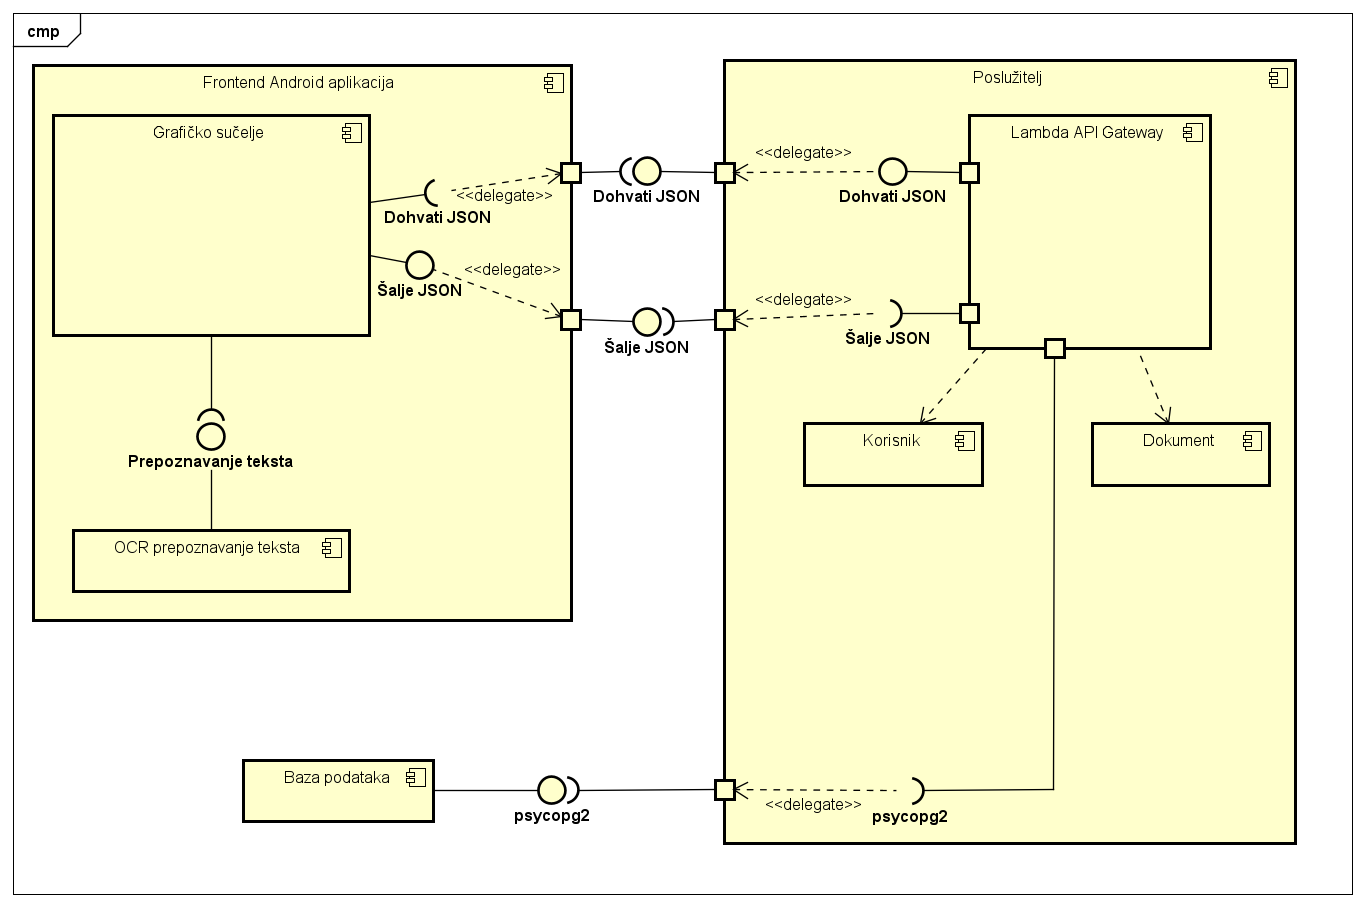
\includegraphics[width=\linewidth]{./dijagrami/Dijagram_komponenti.png}
			 	\caption{Dijagram komponenti}
			 	\label{fig:DK}
			 \end{figure}